\documentclass[10pt,onecolumn]{article}
\usepackage{graphicx}
\usepackage{hyperref}
\usepackage{url}
\usepackage{wrapfig}
\usepackage{tikz}

\title{\vspace{-4.2cm}Software Requirement Specification for Tracking Interconnected Facebook Links }
\author{ ELEN4009 - Software Engineering\\ Julian Zeegers (704582) \\  Joseph Gage (751052)\\ James Allingham (672732) \\ Nathan Haag (873666)}

\addtolength{\oddsidemargin}{-1.5cm}
\addtolength{\evensidemargin}{-.0cm}
\addtolength{\textwidth}{3cm}


%%%%%%%%%%%%%%%%%%%%%%%%%%%%%%%%%%%%%%%%%%%%%%%%%%%%%%%%%%%%%%%%%%%%%%%%%%%%%%%
\begin{document}
\date{\vspace{-5ex}}
\maketitle
\pagestyle{plain}
\setcounter{page}{1}

%%%%%%%%%%%%%%%%%%%%%%%%%%%%%Main Body%%%%%%%%%%%%%%%%%%%%%%%%%%%%%%%%%%%%%%


\section{Introduction}
The Tracking Interconnected Facebook Links project is a project that  is intended to visualize the links and connections of a Facebook user with other users. Initially, these visualization are focused on identifying the relationships of a Facebook user (and the end user of this product) with the network of friends this Facebook user has. The visuals are also intended to further illustrate the relationship connections of the users friends of friends and an overview of the user's friend network. There will be more features that could potentially be added to this tool and therefore the solution must be dynamic and flexible. This document describes the software requirements that will ensure that the end product is of the highest quality, produced most efficiently and is created as close to the requirements as possible.

\subsection{requirements}

The requirements for the application are that it:
\begin{enumerate}
\item consists of a front-end that runs client side and a back-end that runs server side 
\item has user friendly friendly front-end which is easy to use for non-technologically inclined people
\item is scalable - with a back-end that supports multiple clients
\item is fast and responsive leading to a pleasant user experience
\item provides attractive and useful visualisations of Facebook data which allow the user to explore their Facebook networks in an intuitive and practical manner leading to new and interesting discoveries being made
\item is extensible - allowing for additions and modifications to be made quickly and with ease
\item is secure - keeping the users personal data safe and respecting their privacy
\item allows flexibility for data acquisition - the application should allow users to upload their own data or access their data via the Facebook API
\end{enumerate}

\subsection{System Overview}
This project will be made up of various software systems with the back-end and front-end working together to form a dynamic visualization program. The overview of the entire software system is illustrated in Figure 1. This figure shows how the various components of the system interact with each other. Figure 1 shows how the client (using a web browser) interacts with an Apache server and the Django framework. It also shows that the Neo4j database provides data to the framework and is then sent to the web browser (through the Apache server) to create visualizations.

\begin{figure}[h]
	\centering
	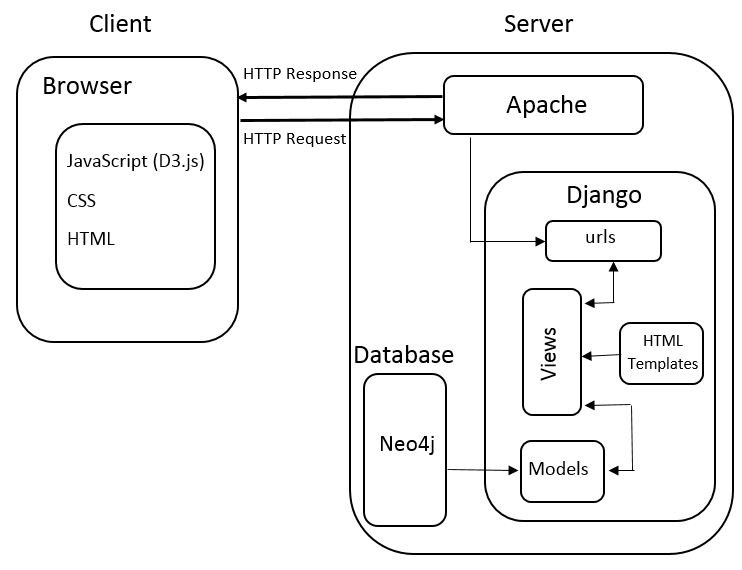
\includegraphics[scale=0.65]{system.jpg}
	\caption{Diagram of System Overview}
	\label{system}
\end{figure}

\section{Software Development Life Cycle Choice}
The Software Development Life Cycle (SDLC) is the process or approach the software development team adheres to throughout the project's development. Choosing the correct SDLC of the project is an important decision at the start of a software project as it could determine whether a project is successfully completed in the time given and at the required quality. There are a few SDLCs that are taken under consideration such the sequential development Waterfall approach or the Iterative and Incremental process in which features are gradually added. However, for this particular project, the fast pace method of the Agile SDLC was thought to be the best approach as the pace of producing a working solution is a priority. The requirements for this project is also not fully defined and therefore the chosen Agile SDLC must be flexible and able to deal with slight requirement changes.

The Agile SDLC also has varying methodologies that allows the achievement of an agile software development movement. These methods include the Dynamic System Development Method, the Scrum Method and the Feature-Driven Development Method. The Scrum methodology is the chosen method for this project as it allows the project progression to be agile and flexible with continuous feedback sessions to ensure the requirements are dynamical followed\cite{Kinsey}.

In the Scrum process, prioritized project tasks (referred to as sprints) are defined in short daily meetings (typically 15 minutes) with all the project team members. These meetings allow the team to communicate project progress and identify the important features that need to be added in order to increase the project progress pace. For the Tracking Interconnected Facebook Links project, these sprints will allow for a working product to be produced in the shortest amount of time while additional features can be  added at a later stage. This process also allows the client to closely keep track of progress and adjust the requirements in order to produce the most high-grade product possible. The daily meeting process occurs for up to 30 days by which time the first release of the developed software should be ready.   


\section{Architecture Choice}


\section{Front-end User Interface Method}


\section{Back-end Service}

The back-end will be based on the \emph{Django} web framework running on an \emph{Apache Web Server}. The DBMS will be \emph{Neo4j}, a graph database, that will be interacted with via the Python driver \emph{Py2neo}. 
\subsection{Django}
\begin{wrapfigure}{r}{0.2\textwidth}
  \begin{center}
    
\includegraphics[width=0.18\textwidth]{django}
  \end{center}
  \caption{The Django Logo}
\end{wrapfigure}


Django is an open source high-level Python Web Framework. It is based on speed, security and scalability. It is also commonly used, with companies such as Mozilla, Pinterest and National Geographic building their websites with it \cite{django}. 

Although it has its own nomenclature, Django can be considered an MVC (Model View Controller) framework and has been compared to the popular \emph{Ruby on Rails} web framework. An MVC framework is based on a three layer abstraction. The first layer abstracts the data access of the web application and is called the Model layer. The second layer is responsible for data display and is called the View layer. The final layer regulates the Views and is called the Controller layer. In Django's nomenclature, the view is equivalent to the standard controller, the template is equivalent to the standard view and the model is much the same as usual. For this reason Django is often referred to as a MTV or Model Template View framework \cite{djangobook}. It is important to note that Django is not a programming language, it is a programming pattern designed to streamline web development in the Python programming language.

Django has its own lightweight web server designed to be used for testing and development. However, for production the Django Software Foundation recommends using Apache with the \emph{mod\_wsgi} module \cite{djangoApache}.
\subsection{Apache}

Apache is a free HTTP web server that has been in production since 1995. It is an extremely sophisticated and flexible tool which supports the newest HTTP standards and a large number of platforms \cite{apache}. Apache has a large number of compiled modules that greatly extend it's functionality. 
\begin{wrapfigure}{r}{0.2\textwidth}
  \begin{center}
    
\includegraphics[width=0.18\textwidth]{apache}
  \end{center}
  \caption{The Apache Logo}
\end{wrapfigure}


Apache processes any incoming HTTP requests from the clients and then sends the appropriate HTTP responses back. This will be done by interfacing with the Django web framework which will make the appropriate decisions based on the requests, and return responses containing content such as information from the Neo4j database. 

Apache has many functions such as virtual hosting which allow one Apache installation to server multiple websites. This feature allows developers of small websites to save on server costs. Apache also provides many useful security features required when a website goes into production such as: password and digital certificate authentication, SSL and TLS support, and many more. For larger websites Apache also allows load balancing. 

\subsection{Neo4j}
Neo4j is a graph database written in Java. It is widely used and has drivers for many languages including Python. Neo4j follows the Atomicity Consistency Isolation Durability (ACID) model which means that it is extremely reliable.  

Graph databases are a type of NoSQL or Not Only SQL database. They excel at managing large complex sets of data which can be described as nodes and relationships. Figure \ref{neo4eg} shows an example of the type of data that can be stored in a graph database.

\begin{figure}[htbp]
    \centering
    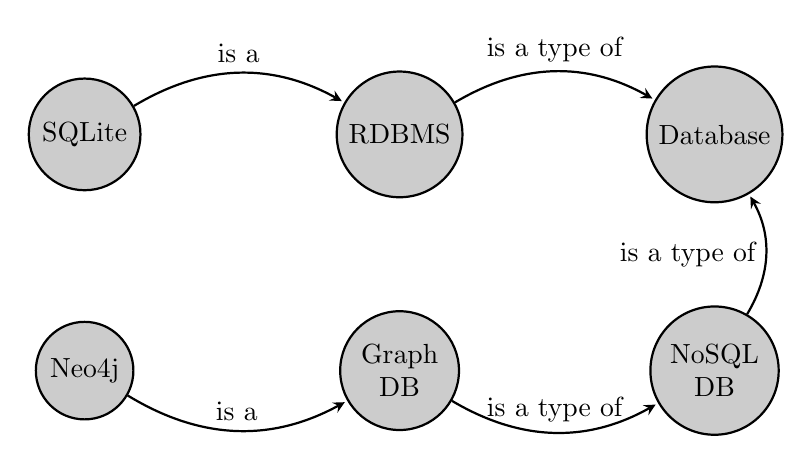
\begin{tikzpicture}[->,>=stealth,shorten >=1pt,auto,node distance=3cm,
       thick,main node/.style={circle,fill=black!20,draw,align=center}]

      \node[main node] at (0,0) (1) {Neo4j};
      \node[main node] at (4,0) (2)  {Graph\\ DB};
      \node[main node] at (8,0) (3) {NoSQL\\ DB};
      \node[main node] at (8,3) (4) {Database};
      \node[main node] at (4,3) (5) {RDBMS};
      \node[main node] at (0,3) (6) {SQLite};
      \path
      (1) edge [bend right] node {is a} (2)
      (2) edge [bend right] node {is a type of} (3)
      (3) edge [bend right] node {is a type of} (4)
      ;
      \path 
      (6) edge [bend left] node {is a} (5)
      (5) edge [bend left] node {is a type of} (4)
      ;

    \end{tikzpicture}
    \caption{Example of data stored in a graph database}
    \label{neo4eg}
\end{figure}

In this application the data being stored will be that of Facebook relationships. Graph databases are orders of magnitudes faster than a RDBMS for queries on this kind of data, such as finding extended friend networks of individuals \cite{graphdbs}.  Figure \ref{friends} shows an example of the kind of data that will be stored in the database.

\begin{figure}[htbp]
    \centering
    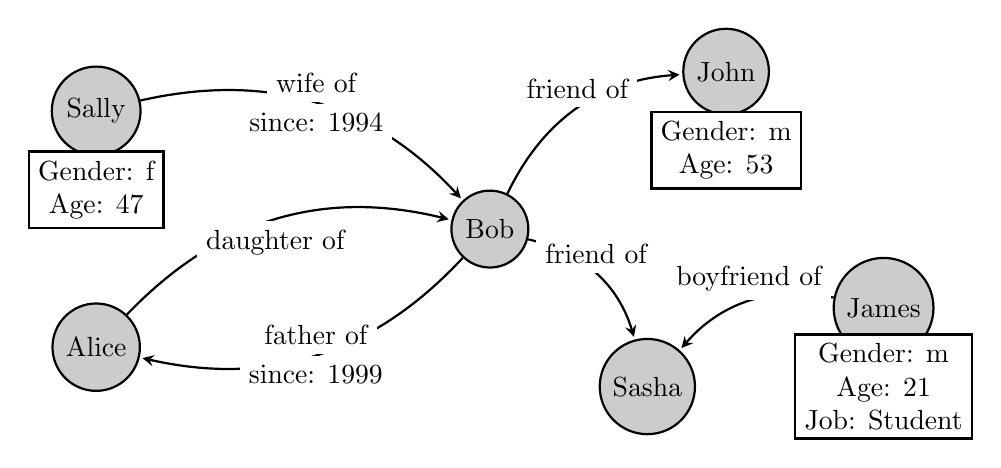
\begin{tikzpicture}[->,>=stealth,shorten >=1pt,auto,thick,main node/.style={circle,fill=black!20,draw,align=center}]

      \node[main node] at (-1,-0.5) (1) {Sally};
      \node[draw,rectangle, below of = 1, align=center,fill=white] (7) {Gender: f\\ Age: 47};
      \node[main node] at (7,0) (2)  {John};
      \node[draw,rectangle, below of = 2, align=center, fill=white] (6) {Gender: m\\ Age: 53};
      \node[main node] at (4,-2) (3) {Bob};
      \node[main node] at (-1,-3.5) (4) {Alice};
      \node[main node] at (6,-4) (5) {Sasha};
      \node[main node] at (9,-3) (8) {James};
      \node[draw,rectangle, below of = 8, align=center, fill=white] (9) {Gender: m\\ Age: 21\\ Job: Student};

    
      \path
      (1) edge[bend left] node[above, fill=white] {wife of} node[below,fill=white] {since: 1994} (3)
      (3) edge[bend left] node[above,fill=white] {friend of} (5)
      (3) edge[bend left] node[above,fill=white] {father of} node[below,fill=white] {since: 1999} (4)
      (3) edge[bend left] node[above,fill=white] {friend of} (2)
      (8) edge[bend right] node[above,fill=white] {boyfriend of} (5)
      (4) edge[bend left] node[below,fill=white] {daughter of} (3)
      ;

    \end{tikzpicture}
    \caption{Example of facebook type data in a graph database}
    \label{friends}
\end{figure}
Note, from Figure \ref{friends}, that both the relationships as well as the entities themselves have associated data. In face each entity acts as a key value store. Queries can be performed to find all friends since a certain date or all friends of friends (as discussed above). These queries can be performed using Neo4j's \emph{Cypher} query language or via language drivers. The language driver that will be used for this application is Py2neo.

\section{Supporting Software}
The Interconnected Facebook Links project is intended to be used by a Facebook user and this user is assumed to not technically advanced. Therefore the final product needs to be user friendly and easy to use. The supporting software mentioned in this section describes the technologies that will be used to ensure the user-friendliness and functionality of the product is achieved. The framework and internal structure  of the project in terms of the architecture, front-end and back-end has been described in the previous sections. This section describes the software that will be used to support these mentioned structures.

In order to ensure that the end program is easy to use and looks professional, the visual design and theme needs to have a consistent, well designed layout and be visually attractive. Bootstrap is a HTML, CSS and JavaScript framework that allows this front-end visual design to be achieved \cite{Bootstrap}. Bootstrap provides various templates that will maintain the consistent theme throughout the final created website. It also provides navigational links for the website and the template is customizable so it can be used to create the desired theme. The Bootstrap template that will be utilized is the "dashboard template" as it has a good layout, navigational links and is visually attractive which is taken from \cite{Bootstrap}.

Another technology that will support the functionally of the website is the D3.js JavaScript graphical library (assessed from \cite{D3}). This library contains JavaScript code for many different visualization graphs that can be used to visualize the data stored in the Neo4j database. Considering that the requirements for this project is to visualize the interconnections, the "force-directed graph" from the d3.js library will be used. Due to the fact that the requirements are flexible, other graphs from the d3.js library can also be used to the further visualize the database if the requirements change. These other graphs include dynamic bar and line charts, geographical heatmaps and dc.js crossfilter graphs plus others that will be considered. 

\begin{thebibliography}{1}
\bibitem{Kinsey} H. van Vliet, \emph{Software Engineering: Principles and Practice} Wiley, 2007.
\bibitem{django} Django Software Foundation. \emph{Django Overview}. \url{https://www.djangoproject.com/start/overview/}. 2016. Last accessed: 9 March 2016. 
\bibitem{djangobook} Adrian Holovaty, Jacob Kaplan-Moss, et al. \emph{The Django Book}. \url{http://www.djangobook.com/en/2.0/index.html#}. Ch 3. Last accessed: 9 March 2016.
\bibitem{djangoApache} Django Software Foundation. \emph{How to install Django}. \url{https://docs.djangoproject.com/en/1.9/topics/install/}. 2016. Last accessed: 9 March 2016.	
\bibitem{apache} Apache Software Foundation. \emph{Apache - HTTP Server Project}. \url{https://httpd.apache.org/ABOUT_APACHE.html}. 2016. Last accessed: 9 March 2016.	
\bibitem{graphdbs} Robinson I, Webber J, Eifrem E. \emph{Graph Databases} O'Reilly Media. ch 2. pp 21 - 22. June 2013.
\bibitem{Bootstrap}  \emph{Get Bootstrap - 3.3.6} \url{www.getbootstrap.com} Last accessed: 9 March 2016.
\bibitem{D3}  \emph{D3.js - Data Driven Documents} \url{www.d3.com} Last accessed: 9 March 2016.


\end{thebibliography}

 %%%%%%%%%%%%%%%%%%%%%%%%%%%%%%%%%%%%%%%%%%%%%%%%%%%%%%%%%%%%%%%%%%%%%%%%%%%%%%
\clearpage
\end{document}
